\documentclass{article}
\usepackage{graphicx} 
\usepackage[dutch]{babel}
\usepackage{graphicx}
\graphicspath{ {./images/} }
\begin{document}
\sffamily



\begin{titlepage}
  \centering
    \vfill
    {\bfseries\Huge
      Verslag Tinlab Advanced Algorithms \\
        \vskip2cm
      }
      {\bfseries\Large
        S. T. Udent\\
      }
      {
        \bfseries\normalsize
        176-671\\
        \vskip1cm
        \today\\
    }    
    \vfill
    
\includegraphics[width=4cm]{logohr.png} % also works with logo.pdf
    \vfill
    \vfill
\end{titlepage}
\newpage
\tableofcontents

\newpage
\section{Inleiding}
In dit document wordt uitleg, voorbeelden en uitwerkingen van oefeningen beschreven. 


royce waterfall method



Onderwerp(en): 
Nucleaire testen op het eiland Bikini Atoll.
vlucht 1951 mode confusion turkish airlines
kannon met dubbele loop, John Gilleland
Tsjernobly 1986
ariane 5 64 bit getal wrong format

Context:
bikini eilanden, bom die 5 megaton hogere yield had dan verwacht. vakkennis was er nog niet wat betreft physika om dit te kunnen voorspellen.


World vs. machine:



4 variablen methode:


Mode confusion 
%\cite{bredereke2002rigorous}, //geeft definitie van mode confusion.




\section{test}
test
\subsection{testing}
testing
\section{Requirements}

In dit hoofdstuk wordt er over requirements en specificaties aangeduid. De definities voor deze termen zijn die in dit document zullen worden aangehouden zijn die van %\cite{gunter2000reference}. \newline

\subsection{Requirements}

Requirements beschrijven fenomenen uit de buitenwereld die het probleem beschrijven. \newline
- vragen stellen / survey \newline
- observeren \newline
- brainstormen \newline
- ervaring / literatuurstudie \newline
- specialist raadplegen \newline


\subsection{specificaties}

Specificaties zijn de eisen waaraan de oplossing of product aan moet voldoen en mee wordt geëvalueerd.

\section{Modellen}

\subsection{De Kripke structuur}

Belangrijke termen states en transities.

\begin{figure}[!h]
	\centering
	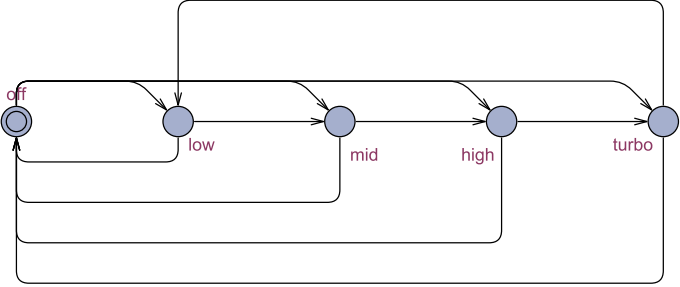
\includegraphics[width=\textwidth]{kripke_structure_example1}
    \caption{Voorbeeld Kripke structuur}
	%\label{fig:figure2}
\end{figure}

\subsection{Soorten modellen}

\textbf{World vs. machine:}
requirements en vereiste.
\textbf{4 variabelen methode:}

Modellen voor computer systemen gebruiken vaak antropomorfisme analogie en intuïtieve conclusies wat tot lager precisie kan leiden. Het vier variabelen model helpt om software vereisten met groter precisie vast te stellen, door deze te modelleren op een manier zoals vaak door ingenieurs wordt toegepast. \cite{parnas1995functional} 

Input/output/gecontroleerde variabelen/gemonitorde variabelen.
\begin{figure}[!h]
	\centering
	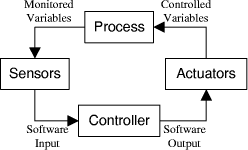
\includegraphics[width=\textwidth]{four_Variables}
    \caption{Vier variabelen model \cite{thompson2000requirements}}
	%\label{fig:figure2}
\end{figure}

\subsection{Tijd}
//Behandeld in week 2
\subsection{Guards en invarianten}
//Behandeld in week 2

\subsection{Deadlock}

\subsection{Zeno gedrag}
//Behandeld in week 2
\section{Logica}

\subsection{Propositielogica}

\subsection{Predicatenlogica}

\subsection{Kwantoren}

\subsection{Dualiteiten}

\section{Computation tree logic}

\subsection{De computation tree}

\subsection{Operator: AG}

\subsection{Operator: EG}

\subsection{Operator: AF}

\subsection{Operator: EF}

\subsection{Operator: AX}

\subsection{Operator: EX}

\subsection{Operator: p U q}

\subsection{Operator: p R q}

\subsection{Fairness}

\subsection{Liveness}

\newpage
\subsection{Temp log:}
week 1: 
world vs. machine
requirements en specifications
systems engineering vs. software engineering
4 variablen
week2:
tijd
guards en invarianten
deadlocks
week3:

Wat is een goed model? cite the links from powerpoint, first links describes what the dia explains, deze link wordt ook gebruikt om de eindopdracht te beoordelen, eindverslag moet afweging laten zien wat betreft je keuzes, wat zijn je argumenten?

google scholar "to predict and serve?"

een goed model moet het verschil tusssen ruis en echte informatie kunnen aantonen.

uppaal for sharing int below 5 don't use global variables

ebsilon/absilon-delta stelling wiskunde limiet begrip
\newpage
\bibliography{references}
\bibliographystyle{plain}
\end{document}


